\chapter{Architektura rozwiązania}
\section{Model Widok Prezenter}
Aplikacje internetowe z reguły najlepiej wpisują się we wzorzec MVP (ang. Model-View-Presenter, Model-Widok-Prezenter), z którego autor postanowił skorzystać jako podstawe architektury systemu. Wzorzec ten polega na przekazaniu kontroli nad danymi prezentowanymi przez system do obiektu zwanego Prezenter. Mimo, że zdarzenia bezpośrednio pojawiają się w warstwie widoku, to natychmiast są one przekazywane do Prezentera, który w razie potrzeby odwołuje się do wartswy modelu i ewentualnie zmienia wygląd widoku prezentowanego użytkownikowi.

\begin{figure} [H]
    \begin{center}
	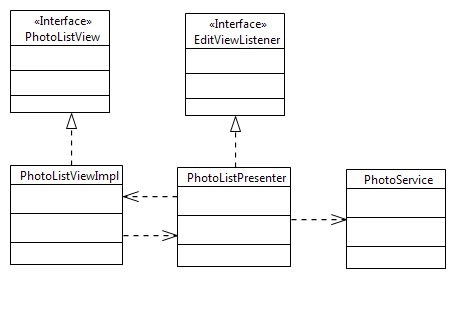
\includegraphics[scale=.8]{img/mvp.png}
	\caption{Przykład implementacji wzorca MVP}
	\label{mvp}
    \end{center}
\end{figure}

Powyższy rysunek przedstawia implementacje wzorca MVP w systemie wspierającym prowadzenie ewidencji badań archeologicznych. Na przykładzie widoku oraz prezentera listy zewidencjonowanych zdjęć pokazana jest współpraca komponentów.

\newpage
Aby maksymalnie rozluźnić zależności między obiektami zastosowane są interfejsy przez które komunikują się Widok z Prezenterem. Prezenter wystawia interfejs, który musi być implementowany przez widok, natomiast widok umożliwia jedynie rejestracje prezentera jako nasłuchiwacza zdarzeń. 

W chwili wystąpienia zdarzenia, np. chęci dodania nowego zdjęcia do listy, widok wywołuje odpowiadającą temu zdarzeniu metode na wszystkich obiektach zarejestrowanych jako nasłuchujące na obiekcie widoku. Prezenter otrzymuje w ten sposób notyfikacje, która może powodować np. komunikacje z baza danych przez obiekt PhotoService (np. dodanie do bazy danych nowego zdjęcia). Na zakończenie przetwarzania prezenter musi powiedzieć widokowi, że zmieniła się lista zdjęć. Aby utrzymać maksymalne rozluźnienie zależności, widok jest powiadamiany przez interfejs który implementuje.

\section{Podzial na pakiety}
Konsekwencją zastosowania wzorca MVP jest rozluźnienie zależności między obiektami, dzięki czemu w prosty sposób da się wyodrębnić luźno powiązane ze sobą moduły. W systemie zostały wyodrębnione 4 podstawowe pakiety:
\begin{itemize}
\item logic - pakiet zawierający definicje prezenterów oraz klas abstrakcyjnych z nimi powiązanych
\item gui - pakiet zawierający definicje widoków oraz klas abstrakcyjnych z nimi związanych
\item data - pakiet przechowujący kod procedur wykonujących operacje utrwalania danych
\item common - pakiet zawierający klasy wspólne dla klas z pakietów logic i gui
\end{itemize}

\begin{figure} [H]
    \begin{center}
	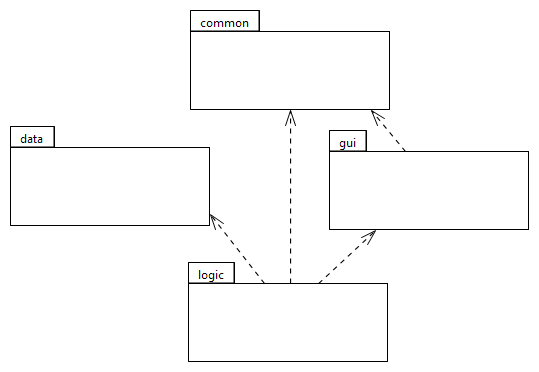
\includegraphics[scale=.6]{img/packageModel.png}
	\caption{Podział klas na pakiety}
	\label{packageModel}
    \end{center}
\end{figure}

\newpage
\section{Nawigacja między widokami}
Szkielet budowy aplikacji Vaadin sam w sobie posiada mechanizm przechodzenia między widokami, jest on jednak dosyć niewygodny w użyciu - istnieje konieczność rejestrowania widoków i ich adresów w momencie inicjalizacji obiektu UI. Na szczęście, dzięki wtyczce SpringVaadinIntegration możliwe jest przechodzenie między widokami jedynie po ich identyfikatorze w kontenerze Spring.

We wspomnianej przeze mnie wtyczce istnieje klasa implementująca powyższe zachowanie - DiscoveryNavigator. Wciąż jednak nie jest ona wystarczająca, jednak po przedefiniowaniu kilku metod okazuje się, że można dostosować ją do swoich potrzeb. 

Rozwiązanie wykorzystane w systemie będącym produktem niniejszej pracy wymaga zarejestrowania widoku w kontrolerze sesji, który na podstawie nazwy widoku nadaje powiązanie z nim odpowiedniemu prezenterowi. Prezenter z kolei, rejestruje się jako słuchacz zdarzeń widoku, którym steruje.

\section{Maksymalna abstrakcyjność}
System wspierający prowadzenie ewidencji dokumentacji archeologicznej musi umożliwiac wprowadzanie wielu rodzajów danych. Wiąże się to z dużą ilością klas z kategorii widoków i prezenterów. Szczególnie w przypadku słowników, istnieje wielka szansa na konieczność wielokrotnego powtarzania tych samych fragmentów kodu, stąd ambicją autora było stworzenie szkieletu aplikacji skracającego czas tworzenia komponentów odpowiedzialnych za wprowadzanie danych do systemu do minimum.

Szkielet aplikacji, o którym była mowa w poprzednim akapicie wymaga dwóch osobnych struktur hierarchii obiektów, jednek dla widoków i jednej dla prezenterów. Konieczne jest także, aby te struktury wzajemniej były od siebie zależne, zgodnie ze wzorcem MVP opisanym w pierwszej części tego rozdziału.

Poniżej zostało zaprezentowane drzewo dziedziczenia widoków, powstałe w wyniku projektu aplikacji, który następnie w trakcie implementacji został delikatnie zmodyfikowany. 

\begin{figure} [H]
    \begin{center}
	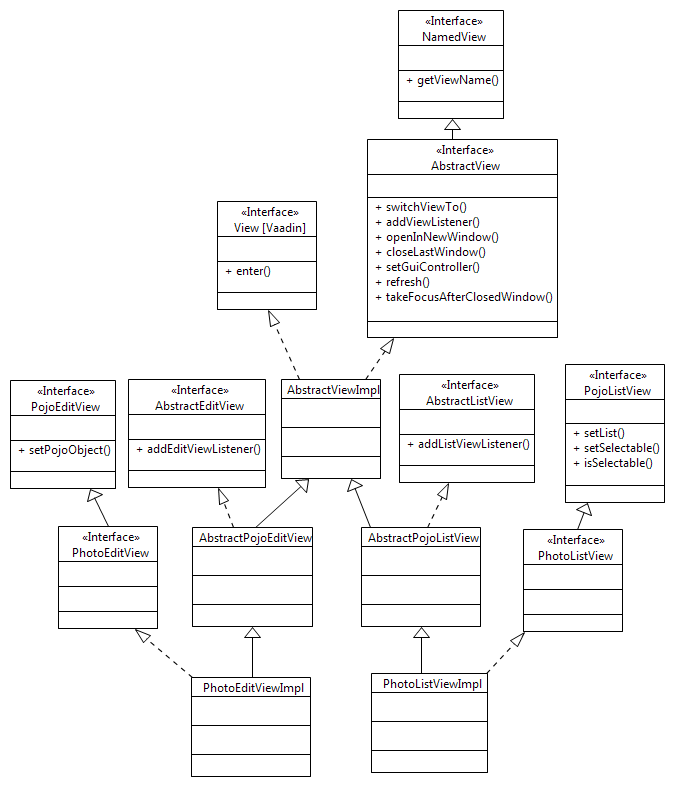
\includegraphics[scale=.55]{img/viewHierarchy.png}
	\caption{Hierarcha widoków}
	\label{viewHierarchy}
    \end{center}
\end{figure}

Na samej górze hierarchii znajduje się interfejs wymuszony przez technologie Vaadin (View), która jest konieczna do wyświetlenia różnych widoków w obrębie jednego obiektu UI. Drugim korzeniem hierarchii jest interfejs NamedView, który pozwala nadawać nazwy widokom, co z kolei utożsamiane jest z nazwą odpowiadającego komponentu Springa (ang. bean) a także przydzielanego fragmentu URI, doczepianego do adresu i pozwalającego przeglądarce zapamiętywać historie nawigacji po stronie.

Całe drzewo dziedziczenia wyraźnie podzielone jest na dwie części - obiekty widoków listy i widoków okna edycji wiersza. Jest to spowodowane oczywiście różnymi zadaniami stawianymi obiektom implementującym powyższe funkcje.

\newpage
Rdzeń implementacji znajduje się w klasach AbstractViewImpl oraz AbstractPojoEditView i AbstractPojoListView. AbstractViewImpl jest klasą z której bezpośrednio dziedziczą wszystkie "standardowe" widoki prezentujące zwykłą treść, np. lista słowników czy strona startowa. AbstractPojoEditView jest z kolei klasą po której bezpośrednio dziedziczą wszystkie implementacje widoków okien edycji użyte w systemie. Implementuje ona wygląd okna edycji (za pomocą klasy DefaultForm, opisanej w rozdziale 7., która dynamicznie generuje wygląd formularza na podstawie adnotacji zawartych w klasie obiektu edytowanego) oraz całą obsługe przekazywania zdarzeń, które zostały wygenerowane przez użytkownika, czyli wywołuje metody na obiektach nasłuchiwaczy (czyli prezenterów).

Warto także dodać, że hierarchia jest skonstruowana w ten sposób, aby uniezależnić maksymalnie reszte klas wchodzących w skład pakietu obsługującego cały interfejs graficzny użytkownika, od technologii prezentacji, którą w tym przypadku jest Vaadin.

\newpage
\begin{figure} [H]
    \begin{center}
	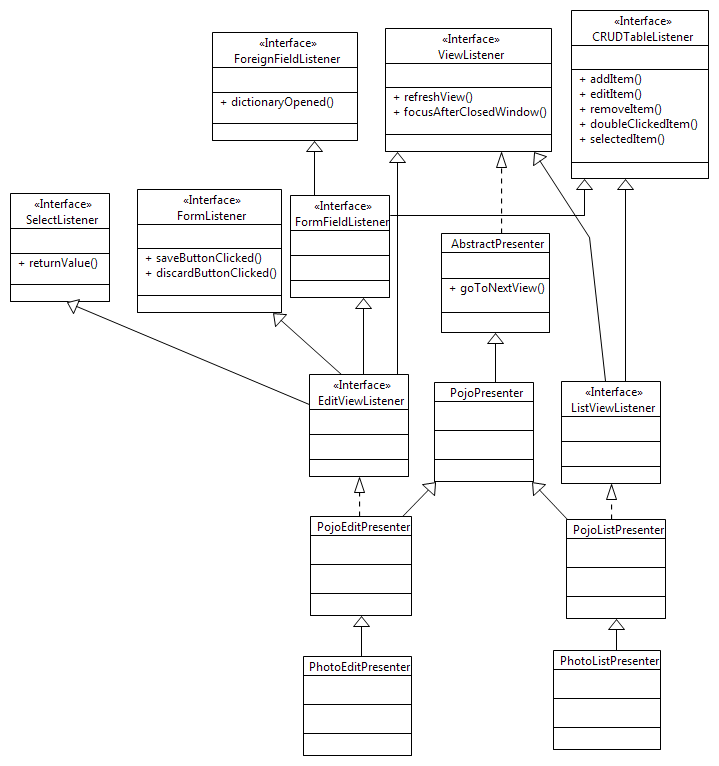
\includegraphics[scale=.6]{img/presenterDiagram.png}
	\caption{Hierarchia prezenterów}
	\label{presenterHierarchy}
    \end{center}
\end{figure}

Powyżej została przedstawiona hierarchia prezenterów w szkielecie aplikacji stworzonym przez autora w trakcie tworzenia systemu ewidencji badań archeologicznych. Na samym początku warto zaznaczyć, że hierarchia ta jest tak rozbudowana, ze względu na dopasowanie do komponentów stworzonych w trakcie pracy nad systemem - ForeignField oraz CRUDTable, które są opisane w rodziale 7.

Dodatkowo, wszystkie widoki użyte w systemie muszą implementować interfejs ViewListener, który pozwala reagować na ogólne zachowania widoków, a mówiąc ściślej, pozwala wykonywać akcje przy okazji przejścia z jednego widoku do drugiego - np. odświerzenie zawartości. 

\newpage
Każdy prezenter w systemie powinien także dziedziczyć po klasie AbstractPresenter, pozwala implementuje elementy związane z nawigacją (pamięta który prezenter jest jego "rodzicem" - czyli jest prezenterem widoku który wywołał ten widok oraz implementuje przejście do następnego widoku).

Tak jak w przypadku hierarchii widoków, tak w przypadku prezenterów konieczne jest rozdzielenie na dwie główne gałęzie - prezenterów okna edycji oraz prezenterów listy obiektów. Gałęzie te mają swoją implementacje kolejno w klasach: PojoEditPresenter i PojoListPresenter. Głównym zadaniem wymienionych klas jest implementacja reakcji na działania użytkownika, które zostały przekazane dalej przez widok poprzez interfejs nasłuchiwacza (zaimplementowany w tych właśnie klasach). Na samym dole hierarchii znajdują się klasy konkretne, odpowiadające prezenterom obiektów dziedziny problemu. Poniżej przykład implementacji prezentera okna edycji:
\begin{lstlisting}
@Component
@Scope("session")
public class FigureSubjectEditPresenter 
			extends PojoEditPresenter<FigureSubject>
{
	public interface FigureSubjectEditView 
			extends PojoEditView<FigureSubject>
	{
	}

	@Autowired
	public FigureSubjectEditPresenter(
			FigureSubjectEditView pojoEditView, 
			AbstractServiceInterface<FigureSubject> pojoServ)
	{
		setView(pojoEditView);
		setPojoService(pojoServ);
	}
}
\end{lstlisting}

Jak widać, powyższy kod implementuje się bardzo szybko. Dodatkową prostote autor osiągnął dzięki zastosowaniu kontenera IoC Springa, który wstrzykuje zależności bezpośrednio do konstruktora, za pomocą adnotacji @Autowired. Warto zwrócić uwagę, że każda klasa konkretna definiuje swój odrębny interfejs widoku, który jednak standardowo posiada takie same metody jak wszystkie inne w tej grupie widoków (okno edycji).

\newpage
Klasa przedstawiona na listingu jest prezenterem okna edycji obiektu, który nie posiada ani kolekcji obiektów podrzędnych (związek Jeden-Do-Wielu oraz Wiele-Do-Wielu) ani obiektów pochodzących ze słownika. Jeżeli by tak było, konieczne byłoby zaimplementowanie dodatkowych metod:
\begin{itemize}
\item getDataProvider() - metoda zwracająca obiekt implementujący interfejs DataProvider, używany w kontekście słowników do wypełniania wartości
\item getDictionaryPresenter() - metoda zwracająca, na podstawie argumentu, prezenter używany przez widok powiązany z danym słownikiem
\item getActiveFieldPresenter() - metoda zwracająca, na podstawie argumentu, prezenter używany przez widok powiązany z jednym z obiektów kolekcji (powinien to być Prezenter Listy w przypadku związku Wiele-Do-Wielu oraz prezenter okna edycji obiektu podrzędnego w przypadku związku Jeden-Do-Wielu, np. specyfikacja rysunku).
\item fillValueInOneToManyRel() - metoda, która wzbogaca obiekt zwrócony z potomnego prezentera, o referencje do obiektu prezentowanego
\end{itemize}

Kod prezentera listy obiektów jest niewiele bardziej skomplikowany:
\begin{lstlisting}
@Component
@Scope("session")
public class FigureSubjectListPresenter 
			extends PojoListPresenter<FigureSubject>
{
	public interface FigureSubjectListView 
				extends PojoListView<FigureSubject>
	{
	}

	@Autowired
	public FigureSubjectListPresenter(
			AbstractServiceInterface<FigureSubject> pojoServ, 
			FigureSubjectListView pojoListView,
			FigureSubjectEditPresenter photoSubjectEditPres)
	{
		super(FigureSubject.class);
		setPojoService(pojoServ);
		setPojoListView(pojoListView);
		setPojoEditPresenter(photoSubjectEditPres);
	}
\end{lstlisting}
\newpage
\begin{lstlisting}
	@Override
	protected Criterion getCriterion()
	{
		return null;
	}

	@Override
	protected FigureSubject getEmptyObject()
	{
		return new FigureSubject();
	}
}
\end{lstlisting}
Ten prezenter także zawiera definicje interfejsu widoku, z którym się komunikuje oraz także w tym przypadku użyty został kontener Springa wstrzykujący zależności bezpośrednio do konstruktora.

Dodatkowo pojawiły się dwie proste metody:
\begin{itemize}
\item getCriterion() - zwracająca kryterium służące do wyboru listy elementów prezentowanych
\item getEmptyObject() - tworzący nowy obiekt, zgodnie ze wzorcem fabryka
\end{itemize}

Jak widać na przykładach powyżej, cała implementacja reakcji prezenterów na zdarzenia przychodzące z interfejsu graficznego użytkownika jest zaimplementowana w klasach abstrakcyjnych, natomiast w klasach konretnych zostało jedynie ustawienie wartości konkretnych pól a także zaimplementowanie odpowiednich abstrakcyjnych metod, które są użyte w klasach abstrakcyjnych.
% ex: set tabstop=4 shiftwidth=4 softtabstop=4 noexpandtab fileformat=unix filetype=tex spelllang=pl,en spell: